%! TeX program = lualatex
\documentclass[10pt,a4paper,table]{article}

\usepackage{amsmath,amssymb,amsthm,mathtools,amsfonts}
\usepackage{breqn}
\usepackage[utf8]{inputenc}
\usepackage[danish]{babel}
\usepackage[T1]{fontenc}

%%%%%%%%%%%%%%%%%%%%%%%%%%%%%%%%%%%%%%%%%%%%%%%%%%%%%%%%%%%%%%%%%%%%%%%%%%%%%% Fonts

\usepackage{fontspec}
\setmainfont{Times New Roman}
\newfontfamily\garamond[Numbers=OldStyle]{EB Garamond}
\newfontfamily\plantin[Numbers=OldStyle]{Plantin MT Pro}
\newfontfamily\quotefont[Ligatures=TeX]{Linux Libertine O}
\newfontfamily\vest{TRY Vesterbro Regular}
\newfontfamily\vestb{TRY Vesterbro Poster}
\newfontfamily\overp{Overpass}

%%%%%%%%%%%%%%%%%%%%%%%%%%%%%%%%%%%%%%%%%%%%%%%%%%%%%%%%%%%%%%%%%%%%%%%%%%%%%% Colors

\usepackage{xcolor}
\usepackage{transparent}

\definecolor{frbblue}{RGB}{47, 88, 109}
\definecolor{hgred}{RGB}{140, 10, 10}
\definecolor{frbgreenl}{RGB}{162, 202, 137}
\definecolor{frbgreen}{RGB}{28, 85, 66}
\definecolor{frbgrey}{RGB}{243, 245, 242}
\definecolor{postityellow}{RGB}{255, 242, 153}
\definecolor{postitgreen}{RGB}{204, 235, 197}
\definecolor{postitblue}{RGB}{199, 224, 244}
\definecolor{postitpink}{RGB}{248, 203, 214}

%%%%%%%%%%%%%%%%%%%%%%%%%%%%%%%%%%%%%%%%%%%%%%%%%%%%%%%%%%%%%%%%%%%%%%%%%%%%%% Other Graphics

\usepackage{graphicx}
\graphicspath{{./img/}{../img/}}
\usepackage{tikz}
\usetikzlibrary{calc,shadows}
\usepackage{placeins}

\usepackage[pdfborder={0 0 0}]{hyperref}

\usepackage{multicol}
\usepackage{cellspace}
\setlength\cellspacetoplimit{100pt}
\setlength\cellspacebottomlimit{100pt}
\usepackage{tabularx}
\newcolumntype{b}{>{\hsize=\hsize}>{\centering\arraybackslash}X}
\usepackage{siunitx}
\setlength\cellspacetoplimit{4pt}
\setlength\cellspacebottomlimit{4pt}

\usepackage{enumitem}
\usepackage{wrapfig}
\usepackage{caption}
\usepackage{titlesec}

\setlength{\parskip}{0.5\baselineskip}
\setlength{\parindent}{0cm}
\setlist[enumerate]{label=\alph*),left=20pt}

%%%%%%%%%%%%%%%%%%%%%%%%%%%%%%%%%%%%%%%%%%%%%%%%%%%%%%%%%%%%%%%%%%%%%%%%%%%%%% New commands

\newcommand\svar[1]{\newline\textcolor{red}{\textbf{Svar}\\#1}}

\newcommand*\quotesize{20}
\newcommand*{\openquote}
  {\tikz[remember picture,overlay,xshift=-3ex,yshift=-0ex]
    \node (OQ) {\quotefont\fontsize{\quotesize}{\quotesize}\selectfont``};\kern0pt}

\newcommand*{\closequote}[1]
  {\tikz[remember picture,overlay,xshift=2ex,yshift={#1}]
    \node (CQ) {\quotefont\fontsize{\quotesize}{\quotesize}\selectfont''};}

\newcommand{\qm}[1]{``#1''}
\newcommand{\iquote}[1]{\begin{quote}\itshape \openquote#1\hfill\closequote{0ex} \end{quote}}

%%%%%%%%%%%%%%%%%%%%%%%%%%%%%%%%%%%%%%%%%%%%%%%%%%%%%%%%%%%%%%%%%%%%%%%%%%%%%% Sections
\usepackage{chngcntr}

\renewcommand\thesection{\arabic{section}}

\titleformat{\section}[block]
  {\flushright\overp\Large\color{frbgreen}}
  {}
  {0pt}
  {\clearpage EKSTRA}
  [{\color{frbgreenl}\vspace{-1em}\hspace*{-0.165\linewidth}\rule{\dimexpr1.165\linewidth\relax}{0.4pt}\kern1mm}]

\counterwithout{subsection}{section}
\renewcommand\thesubsection{Exercise \arabic{subsection}}
\titleformat{\subsection}[leftmargin]{\bfseries}{}{0pt}{\hspace{-5em}\thesubsection}

%%%%%%%%%%%%%%%%%%%%%%%%%%%%%%%%%%%%%%%%%%%%%%%%%%%%%%%%%%%%%%%%%%%%%%%%%%%%%% Header & Footer

\usepackage{bigfoot}
\DeclareNewFootnote{a}
\renewcommand{\thefootnotea}{\fnsymbol{footnotea}}
\newcommand{\footnotes}[1]{\footnotea[2]{#1}}
\MakePerPage{footnotes}

\usepackage{fancyhdr}
\fancypagestyle{plain}{%
  \setlength{\headheight}{60pt}%
  \setlength{\headsep}{0pt}
  \fancyhf{}
  \renewcommand{\footrulewidth}{0pt}%
  \renewcommand\headrule{}%
  \fancyhead[L]{}
  \fancyhead[C]{}
  \fancyhead[R]{\overp\color{frbgreenl}\normalsize English\\\huge\color{frbgreen}\vestb Subject--Verb Agreement}
  \cfoot{\thepage}
}
\pagestyle{fancy}
\fancyhf{}
\renewcommand\headrule{}
\lhead{}
\rhead{}
\cfoot{\thepage}

%%%%%%%%%%%%%%%%%%%%%%%%%%%%%%%%%%%%%%%%%%%%%%%%%%%%%%%%%%%%%%%%%%%%%%%%%%%%%% Document

\begin{document}
\thispagestyle{plain}
\begin{tikzpicture}[remember picture,overlay]
    \node[anchor=north west,yshift=-48pt,xshift=120pt,opacity=0.2]%
        at (current page.north west)
        {
\includegraphics[scale=0.25]{frbvuc_logo.png}};
\end{tikzpicture}
\begin{tikzpicture}[remember picture,overlay]
  \definecolor{bgline}{RGB}{205,214,208}
  \coordinate (C) at ($(current page.north)+(35mm,-5mm)$);
  \draw[bgline, line width=0.6pt] (C) circle (65mm);
  \draw[bgline, line width=0.4pt]
    ($(current page.north east)+(0,0mm)$) ++(-28mm,0)
    -- ($(current page.south east)+(0,10mm)$) ++(-28mm,0);
\end{tikzpicture}

\subsection{}

\textbf{Læs følgende engelske ordsprog. Afgør, om verballeddene i hvert ordsprog er bøjet i singularis eller pluralis.}

\vspace{0.5cm}

{\renewcommand{\arraystretch}{2.2}
\setlength{\tabcolsep}{8pt}
\noindent\begin{tabularx}{0.96\textwidth}{|>{\raggedright\arraybackslash}X|>{\centering\arraybackslash}p{0.18\textwidth}|>{\centering\arraybackslash}p{0.18\textwidth}|}
\hline
 & \textbf{Singularis} & \textbf{Pluralis} \\
\hline
1. The grass is always greener on the other side of the hill. & $\bigcirc$ & $\bigcirc$ \\
\hline
2. Great minds think alike. & $\bigcirc$ & $\bigcirc$ \\
\hline
3. Good things come to those who wait. & $\bigcirc$ & $\bigcirc$ \\
\hline
4. A journey of a thousand miles begins with a single step. & $\bigcirc$ & $\bigcirc$ \\
\hline
5. A picture is worth a thousand words. & $\bigcirc$ & $\bigcirc$ \\
\hline
6. Actions speak louder than words. & $\bigcirc$ & $\bigcirc$ \\
\hline
7. The apple doesn't fall far from the tree. & $\bigcirc$ & $\bigcirc$ \\
\hline
8. Too many cooks spoil the broth. & $\bigcirc$ & $\bigcirc$ \\
\hline
\end{tabularx}
}

\clearpage
\subsection{}

\begin{center}
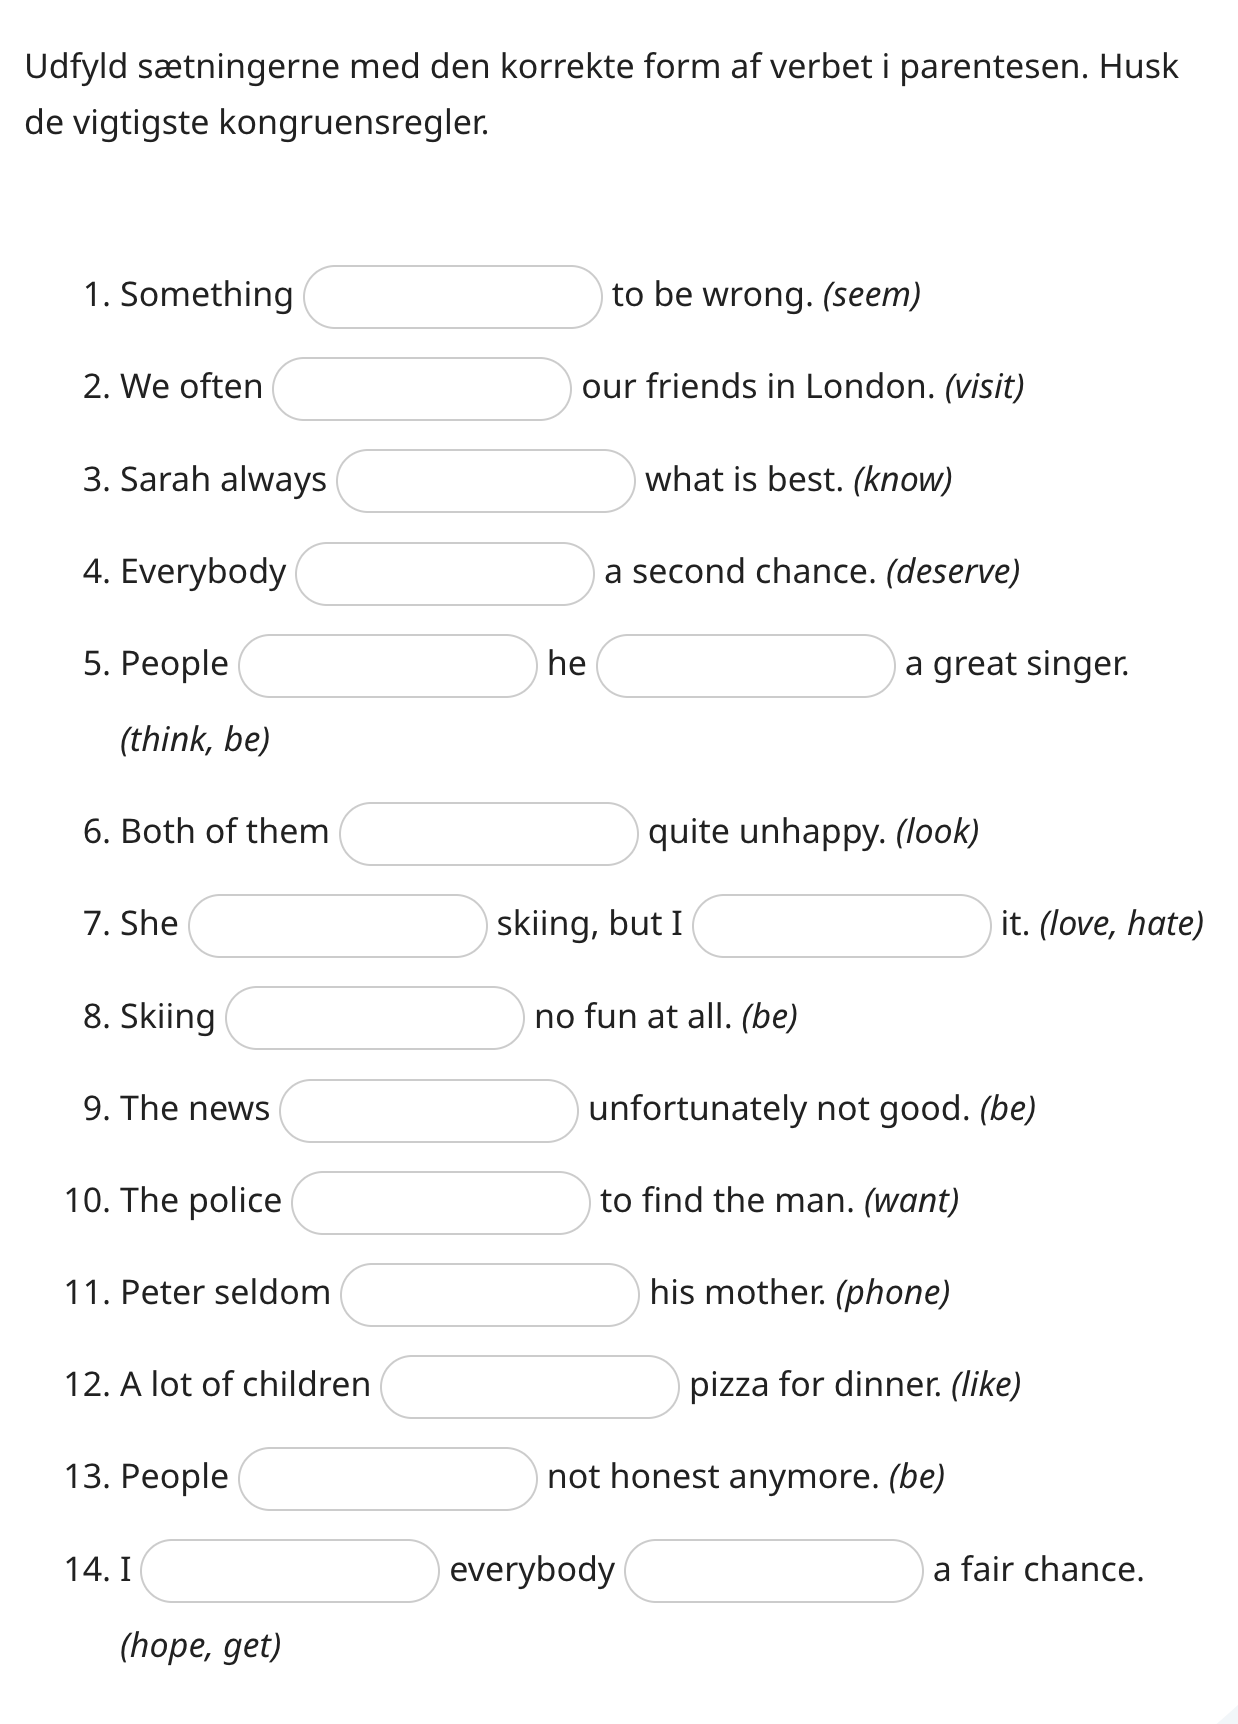
\includegraphics[width=0.92\textwidth]{sva_basics.png}
\end{center}

\clearpage
\subsection{}

\textbf{Ret "fejlene"}\\[-0.2em]
{\small Find 6 kongruens fejl i følgende uddrag af the Adventures of Huckleberry Finn.}
\vspace{0.3cm}

\begin{quote}\itshape
When we was passing by the kitchen I fell over a root and made a noise. We scrouched down and laid still. Miss Watson's big nigger, named Jim, was setting in the kitchen door; we could see him pretty clear, because there was a light behind him. He got up and stretched his neck out about a minute, listening. Then he says:

\qm{Who dah?}

He listened some more; then he come tiptoeing down and stood right between us; we could a touched him, nearly. Well, likely it was minutes and minutes that there warn't a sound, and we all there so close together. There was a place on my ankle that got to itching, but I dasn't scratch it; and then my ear begun to itch; and next my back, right between my shoulders. Seemed like I'd die if I couldn't scratch. Well, I've noticed that thing plenty times since. If you are with the quality, or at a funeral, or trying to go to sleep when you ain't sleepy---if you are anywheres where it won't do for you to scratch, why you will itch all over in upwards of a thousand places. Pretty soon Jim says:

\qm{Say, who is you? Whar is you? Dog my cats ef I didn't hear sumf'n. Well, I know what I's gwyne to do: I's gwyne to set down here and listen tell I hears it agin.}

So he set down on the ground betwixt me and Tom. He leaned his back up against a tree, and stretched his legs out till one of them most touched one of mine. My nose begun to itch. It itched till the tears come into my eyes. But I dasn't scratch. Then it begun to itch on the inside. Next I got to itching underneath. I didn't know how I was going to set still.

Tom he made a sign to me---kind of a little noise with his mouth---and we went creeping away on our hands and knees. When we was ten foot off Tom whispered to me, and wanted to tie Jim to the tree for fun. But I said no; he might wake and make a disturbance, and then they'd find out I warn't in.
\end{quote}

\vspace{0.2cm}

\begin{enumerate}[label=\arabic*.,left=20pt,itemsep=1.2em]
  \item \rule{0.9\textwidth}{0.4pt}
  \item \rule{0.9\textwidth}{0.4pt}
  \item \rule{0.9\textwidth}{0.4pt}
  \item \rule{0.9\textwidth}{0.4pt}
  \item \rule{0.9\textwidth}{0.4pt}
  \item \rule{0.9\textwidth}{0.4pt}
\end{enumerate}

\clearpage
\subsection{}

\textbf{Writing task: subject--verb agreement in context.}

\vspace{0.3cm}

\begin{center}
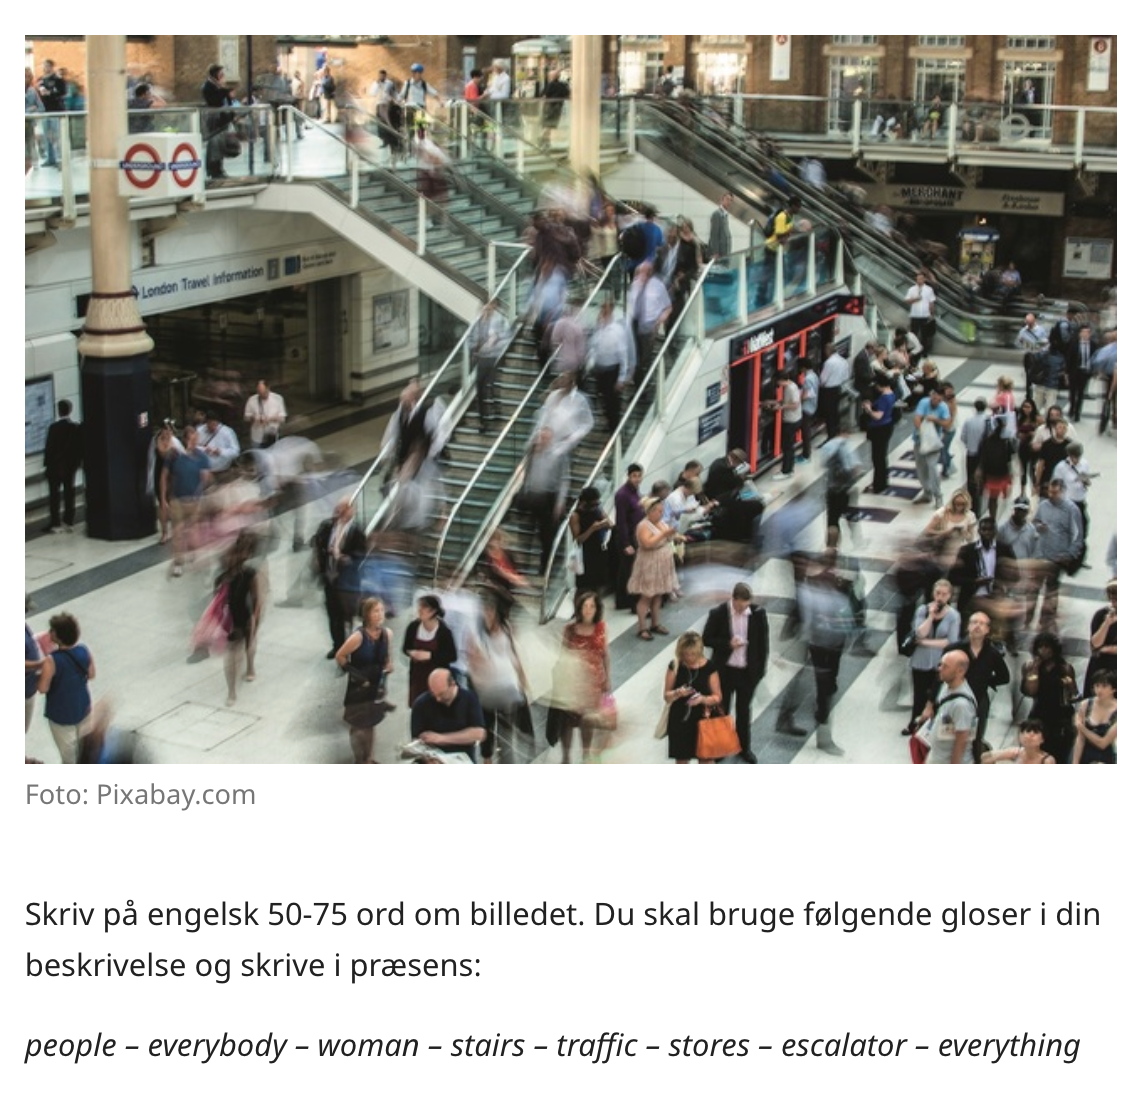
\includegraphics[width=0.92\textwidth]{station_writing.png}
\end{center}

\vspace{0.4cm}

\noindent\rule{\textwidth}{0.4pt}\\[1.1em]
\rule{\textwidth}{0.4pt}\\[1.1em]
\rule{\textwidth}{0.4pt}\\[1.1em]
\rule{\textwidth}{0.4pt}\\[1.1em]
\rule{\textwidth}{0.4pt}\\[1.1em]
\rule{\textwidth}{0.4pt}

% Teacher key:
% Exercise 1: singularis; pluralis; pluralis; singularis; singularis; pluralis; singularis; pluralis.
% Exercise 3 possible SVA corrections: When we were passing; who are you; where are you; I am going; I am going; I hear it again; when we were ten foot off; I wasn't in.
% Exercise 4: writing task. Check especially: people are/have/go; everybody is/has/goes; woman is/has/goes; stairs are/lead; traffic is; stores are/have; escalator is/goes; everything is.

\end{document}
